\documentclass{IEEEcsmag}

\usepackage[colorlinks,urlcolor=blue,linkcolor=blue,citecolor=blue]{hyperref}

\usepackage{color}
\usepackage{listings}
\usepackage{amssymb}
\definecolor{mygray}{rgb}{0.5,0.5,0.5}
\lstset{
numbers=left,
numbersep=5pt,
numberstyle=\tiny\color{mygray}
}
\jvol{XX}
\jnum{XX}
\paper{8}
\jmonth{May/June}
\jname{CiSE}
\pubyear{2019}
\newtheorem{theorem}{Theorem}
\newtheorem{lemma}{Lemma}

\setcounter{secnumdepth}{0}

\begin{document}

\sptitle{Department: Electronic Engineering}
\editor{Editor: Name, xxxx@email}

\title{Reproducing Scientific Experiment with Cloud DevOps}

\author{Feng Zhao}
\affil{Tsinghua University}

\author{Shaolun Huang}
\affil{Tsinghua University}

\author{\textbf{L}in Zhang}
\affil{Tsinghua University}

\markboth{Department Head}{Paper title}

\begin{abstract}
The reproducibility of scientific experiment is vital for the advancement of disciplines based on previous work. To achieve this goal, many researchers focus on complex methodology and self-invented tools which have difficulty in practical usage. In this article, we introduce the DevOps infrastructure from software engineering community and shows how DevOps can be used effectively to reproduce experiments for computer science related disciplines. DevOps can be enabled using freely available cloud computing machines for medium sized experiment and lab HPC environment for large scale computing, thus powering researchers to share their experiment result with others in a more reliable way.
\end{abstract}

\maketitle

\chapterinitial{THE INTRODUCTION} As the development of Big Data and Artificial Intelligence, computational scientific experiments encompass more disciplines and are much more complex than before. Training a useful AI model not only takes long time, consumes large memory but also requires advanced computational device like GPU. Besides, traditional simulation experiment like sequence alignment can be done on new HPC cluster architecture like serveless using more advanced parallel algorithms \cite{niu2019leveraging}. There are also other emerging domains which are related to computational scientific experiment. These experiments require more dedicated toolchains, specific workflow and expensive computational resources which put new challenge on experiment reproducibility.

To solve these issues, there are three kind of approaches: Tools, Platform and Methodology. Many tools \cite{greff2017sacred} are provided, which can capture the running environment information or storing the experiment results. These tools are valuable but may suffer from bad-maintainability and difficult configuration. Indeed, they are made by domain specific scientists, not by experienced full-time software engineers. These tools can store the experiment results, which requires users to configure the database locally. Researchers may not be experienced in database and the local data is difficult to share. Furthermore, most of these tools are not programming language neutral, which means researchers cannot use them in other programming languages. Still, something is better than nothing if researchers use these tools to manage their experiment.

For platform solution, traditionally containerization is used. In recent years, it has been shown that cloud computing is suitable for scientific research purpose \cite{Howe12}. Configuration on cloud environment from scratch is difficult for unexperienced researchers and it is better to use specific cloud service for research purpose. For example, we have Code Ocean or other commercial cloud systems \cite{perkel2018data}, which can tackle the reproducibility problem to some extend. However, their free tier is mean and researchers probably are not willing to pay for extra computational resource. Budget limitation is an important factor when it comes to buying cloud computing resources.

Methodology, or best practice in reproducibility usually discusses the general principals \cite{stodden2014best} or combines tools and platforms to explore the best practice \cite{QashaCW16}. Generally speaking, methodology is hard to follow as they tend to be ideal and the researchers may not be familiar with or have the ability to setup the toolchain used.  

All the above three aspects have pros and cons for experiment reproducibility. The key is how to combine the three aspects to make the best use of their advantages. This is what DevOps tries to solve. This idea is not newly proposed. Boettiger gives a try using Docker container for experiment reproducibility \cite{Boettiger15}.
He also mentioned the DevOps philosophy and acknowledged its limitations.
There are other research projects which borrow the ideas of DevOps to conduct sophisticated experiments \cite{chwalisz2019walker}. These previous researches are valuable but they are limited to specific domain and local environment. 

There are also dedicated system on the cloud, which tries to solve domain specific problem and is related with experiment reproducibility. \texttt{Devops@mech} is developed for a certain institute, which is based on DevOps methodology \cite{philips2019devops}. For public service, we have    RAMP for data science domain \cite{kegl2018ramp} or VCR for computational results indexing purpose \cite{GavishD12}. Though these services are available when corresponding paper is written, they are unavailable now.
Everest, claimed to simplify the use of clouds for scientific computing, is still available but users are required to attach their own resources before actually using it \cite{VOLKOV2017112}.
Just like existing tools, these lab-made services suffer from bad maintenance.

From the above analysis, we see that previous combination of DevOps with scientific experiment has some shortcomings. In this article, we propose Cloud DevOps approach, which uses DevOps from cloud service point of view. It has the following advantages which are not present completely in previous approaches:
\begin{itemize}
	\item High availability of the service and well maintenance of the infrastructure
	\item Easy to use and have flexible configuration
	\item Unlimited Usage and rich computing resource
\end{itemize}
 In the following sections, we will given an introduction to Cloud DevOps and show the feasibility to incorporate existing tools in Cloud DevOps. We then investigate the reproducibility problem in the domain of machine learning and high performance computing (HPC) and given some suggestions by example for the usage of Cloud DevOps. We believe Cloud DevOps can help researchers be more productive in their experiment and help others easier to follow their research. All too often, helping others actually helps yourself.

\section{INFRASTRUCTURE}
Originally, DevOps refers to the software engineering approach to automate the process of building and deploying software product, which is summarized by its two core components ``Continuous Integration and Deployment (CICD)'' \cite{bass2015devops}. 
DevOps service (server) can be self-hosted or centrally hosted. In either way, it requires some other computing machines (called agents or runners) to actually run the jobs submitted. Usually the jobs are not submitted by hand but triggered by an update of code repository. 
DevOps server is quite complex and self-hosted solution is not suitable for sharing results with others. Therefore it is prefered to use public cloud DevOps service, which provides some free time-unlimitted computing power (cloud agent). Besides, self-hosted computing agent (client) can be used if public provided agent is not suitable to reproduce the experiment due to computing resource limitation. In this article, we only consider cloud hosted DevOps service and call them Cloud DevOps for short.

There are some similarities between Cloud DevOps and Everest infrastructure \cite{GavishD12} . Both of Cloud DevOps and Everest allow dynamic provision of computing resources from public cloud service provider and support computing agents attached by users. The computation can be trigger by user when the button is clicked via web interface.
However, Everest suffers from problems mentioned in the last Section. From the workflow management point of view, Cloud DevOps is similar to Pegasus system \cite{Pegasus}. While the latter is more suitable for large scale distributed computing management, Cloud DevOps is scalable and covers the need from small experiment to large scale experiment as well.

% notebook approach 
There are many freely available Cloud DevOps service for open source project which greatly powers individual developers and open source community. {\bf Table} \ref{tab1} gives some famous providers with the list of their features.

\begin{table}
\caption{Comparison of Cloud DevOps provider (until 2019)}
\label{table}
\small
\begin{tabular}{|m{0.8cm}|@{\hspace{0.3em}}>{\centering}m{0.8cm}@{\hspace{0.8em}}|>{\centering}m{0.8cm}|>{\centering}m{0.8cm}|>{\centering}m{0.8cm}|c|}
\hline
& 
{\scriptsize AppVeyor }& 
 {\scriptsize Azure pipelines} & {\scriptsize CircleCI } &  {\scriptsize GitLab CICD} & {\scriptsize Travis}\\
\hline
 {\scriptsize Platform} & {\scriptsize Windows, Linux} & All & All & Linux docker & All \\
\hline
 {\scriptsize Parallel} & 1 & 10 & 4 & 8 &  5 \\
 \hline
 {\scriptsize  Selfhost } & Y & Y & N & Y & N \\
 \hline
 {\scriptsize Artifact} & N & Y & Y & Y & N \\
 \hline
\end{tabular}
\label{tab1}
\end{table}

In Table \ref{tab1}, "Platform" row summarizes what kinds of operating system (OS) are supported; "Parallel" row represents the maximum number of allowed parallel jobs; "Selfhost" row means whether the service provider supports connection of self-hosted agent; "Artifact" row means whether it supports preservation of job artifacts. Our approach is not limited to a specific DevOps cloud service provider. Instead, we focus on the methodology, which is applicable to almost any service provider.

We call a DevOps infrastructure cross-platform (\texttt{Platform = All} in Table  \ref{tab1}) if it supports Windows, MacOS and Linux 
%(usually Ubuntu) 
OS.
Cross-platform is an important topic in software engineering. For scientific community, most research experiments can only be reproduced on specific version of one Operating System. This is OK since researchers may not have machines of other Operating Systems or have time to make their code run on different platforms. A recent study found a flaw of Python script in an article published on Nature which produces different results on different OS \cite{bhandari2019characterization}. This incident can be avoided if researchers test their experiment code on different OS. Cloud DevOps provides easy configuration for different environments and researchers are encouraged to test their code on different OS without learning too much new knowledge and spending too much time. To the least extent, researchers can choose the most similar environment on the cloud to their local development environment and make the experiment able to run on cloud. To the largest extend, it is beneficial if newly developed algorithms and experiments can be run on more platforms.

Parallelism is a valuable capability on Cloud DevOps. In software engineering community, it is often used to run different tests in parallel.
Artifacts are build product which are ready to be deployed to other places.
Some DevOps service provider give the opportunity to save artifacts permanently. For scientific experiment scenario, independent experiments can be run in parallel jobs and the results (like figures) can be saved automatically for each job and viewed by public.

Cloud DevOps uses configuration file to determine the running environment and workflow instructions. 
Usually the configuration file is written in \texttt{YAML} format. Different Cloud DevOps providers have different schema, but they all do the same thing. Below we give a short introduction of how to configure Cloud DevOps to run the experiment.
\subsection{Choosing Environment for Agent}
Users first choose the actual running environment of their code. Usually, it is the combination of the following items:
\begin{enumerate}
\item virtual machine or docker container.
\item public cloud service or local runner.
\item programming language and version.
\end{enumerate}

For example, on Travis users can have  \texttt{Ubuntu 16.04 Python 3.6} environment by simple requires it in the following way:
\begin{lstlisting}[caption={environment configuration}]
os: linux
dist: xenial
language: python
python: 3.6
\end{lstlisting}

In this configuration, we use the Linux virtual machine provided by cloud service. We also fix the version of certain software. 
Such shortcut makes installing dependency in later workflow management much easier as we do not need to install \texttt{Python} or other pre-installed softwares manually.

Besides virtual machine, many DevOps infrastructures support Docker containers as well, which provides more flexible way to configure the environment. Generally speaking, virtualization is better than bare metal OS for experiment reproducibility \cite{Howe12}. Hence Cloud DevOps can do a good job by providing out-of-the-box virtual machine.

Usually Cloud DevOps is used in cooperation with a source code repository. The system diagram in \textbf{Figure} \ref{fig:principal} shows the interaction between the computing agent, the Cloud DevOps server and the code repository. When the source code is updated, Cloud DevOps server fetches the latest code automatically and trigger the computing agent to run the build. The agent uploads the log file and artifacts to the server after it finishes tasks. The artifacts can be figures of experiment result which will be included in the paper. 
The code repository is used for version control and each running of the agent produces a log file. The source code version and the log file are 1-to-1 correspondent. Inspecting the public available log and its corresponding source code help others to reproduce the same result using public available build machine or on local workstations.

\begin{figure}[!ht]
\centerline{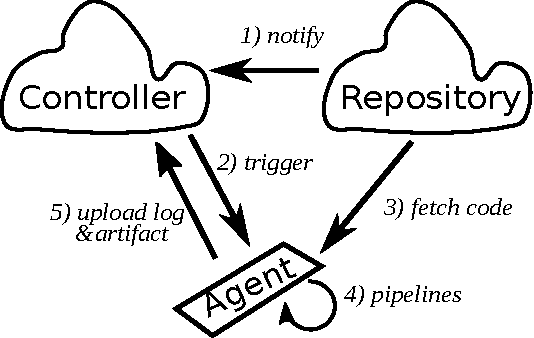
\includegraphics[width=18.5pc]{principal.pdf}}
\caption{Interaction of DevOps server with agent and code repository}\label{fig:principal}
\end{figure}

Though we can use the cloud computing resources for unlimited time, the algorithm level parallel ability is restricted and special computing device (like GPU) or infrastructure (MPI) is missing. The ability to use self-hosted environment is important to run complex scientific experiment. Fortunately, many Cloud DevOps service provides the local agent option to make it possible. By installing a client software, it is possible to empower the advantages of Cloud DevOps without losing the computing ability of lab servers. 
\subsection{Describe Workflow for Agent}
In this step, users should determine how to execute their code sequentially. The basic workflow can be summarized in \textbf{Figure} \ref{fig:cicdworkflow}.

\begin{figure}[!ht]
\centerline{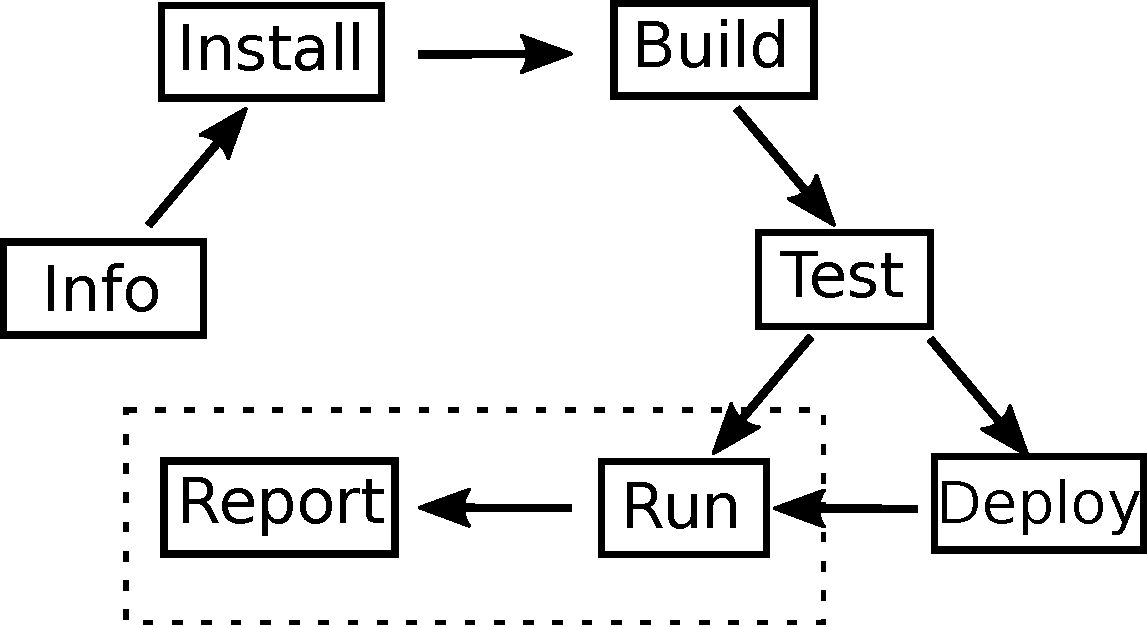
\includegraphics[width=18.5pc]{workflow.pdf}}
\caption{CICD pipeline illustration. The steps within blue boxes are specific stages for scientific experiments. }\label{fig:cicdworkflow}
\end{figure}
%\item build artifact or have deployment stage
%\item build artifact or have deployment stage

The first few steps are common. We need to capture enough information of the running machine (\texttt{Info}) and install necessary software dependencies (\texttt{Install}). Then we build our source code to binary executable (\texttt{Build}) and run some test to verify whether it works for simple cases (\texttt{Test}). In software engineering community, DevOps ends with the deployment step. But for scientific experiment, the story just begins after packing your algorithm to a reusable package. Therefore, we use blue boxes to emphasis the unique steps for scientific experiment in Cloud DevOps infrastructure. After the test, we begin to run the experiment (\texttt{Run}) and finally the result needs to be collected and further processed to produce the artifacts (\texttt{Report}).

For \texttt{Info} step, it is automatically done by DevOps server. For other steps, shell scripts are used to tell the running machine how to install, build and run the code. Not all steps are necessary. For example, no \texttt{Build} step is needed for interpreted programming language. Suppose a researcher writes his experiment code using Python programming language, then he can write his workflow as follows:
\begin{lstlisting}[caption={workflow description}, label={lst:wd}, basicstyle={\small}]
install: 
  - pip install -r requirements.txt
script: # run experiment
  - python main.py
\end{lstlisting}

In the above workflow description, \texttt{Build}, \texttt{Test} and \texttt{Deploy} steps are omitted. This is common for many researchers, often they do not test and deploy their code. That's OK as long as the experiment results are all right. Still, it is better to do some test and do some deployment task. Deployment makes other researchers easier to compare their results with your method without copying your code to their own repository and add input and output wrapper manually.

%Also, DevOps can be customized by self hosting the server in the laboratory or using local runner on workstation or HPC cluster.
Since the configuration of Cloud DevOps is transparent to all users and the mechanism of it is totally determined by configuration file and specific version of source code. Other researchers can trust the output logs and artifacts of DevOps as evidence of experiment reproducibility. Rerunning the code is very easier: just use the same service provider and the code can be run under a different account after replicating the code repository. We acknowledge that this convenience is not applicable to self-hosted agent. For self-hosted agent usually the environment configuration part is not written in a file but determined by which type of agent attached. This made reproducibility less easy. Still, the logs and artifacts are available to be examined by public since they are uploaded to public Cloud DevOps server from local lab agent. To make the story of experiment reproducibility complete,
we encourage the researchers to run a partial and small scale experiment on public DevOps server and run their full experiment on self-hosted server using the same code base. 

\section{CASE STUDIES}
In the previous section, we briefly overview the common practice in DevOps and how it can be related with scientific experiment reproducibility. Different domains may still face different problems in practice. In this section, we show how Cloud DevOps can be used to solve the experiment reproducibility problems in the domain of Machine Learning and High Performance Computing. We believe Cloud DevOps can be used in experiments of other domains as well. 

\subsection{Machine Learning}
Experiment Reproducibility is argued in ML community from different perspectives \cite{kegl2018ramp}. We notice that a platform called Sotabench, similar to DevOps service but dedicated to Deep Learning Reproducibility, has been online in recent month. Currently it only runs the prediction steps for limited public dataset. For more general domains of machine learning, it is preferable to use more simple and flexible approach to resolve the reproducibility problem. In this subsection, we consider some aspects of reproducibility using examples in the domain of machine learning. 

For Machine Learning domain, the workflow shown in Fig \ref{fig:cicdworkflow} can be further decomposed into two phases:
algorithm library build phase and experiment running phase. The output of the first phase is the reusable library which is one of input to the second phase. Using DevOps in the first phase is nearly identical to DevOps used in software community.  The code can be tested against different environment and 
the reusable library can be deployed to public available package repository. For example, in Python programming language, the platform of deployment is \url{pypi.org}. {\bf Table} \ref{tab:deploy} shows the deployment of a Python extension to pypi using DevOps. The deployment result shows that this library supports two versions of Python in a cross-platform way.
\begin{table}
\centering
\begin{tabular}{|c|c|c|c|}
\hline
OS & py3.6 & py3.7  & provider badge\\
\hline
Windows & \checkmark & \checkmark  & 
\includegraphics[width=2cm]{./appveyor.pdf}\\ 
\hline
MacOS & \checkmark & \checkmark & 
\includegraphics[width=2cm]{./travis.pdf}\\ 
\hline
ManyLinux & \checkmark & \checkmark & same as above \\
\hline
\end{tabular}
\caption{cross-platform deployment matrix of a compiled algorithm used in scientific experiment}\label{tab:deploy}
\end{table}

For the experiment running stage, we can just install the deployed package and run the actual experiment. The workflow specification for this stage can be the same with Listing \ref{lst:wd}. In \texttt{requirements.txt} file, we put the package name of our algorithm and other dependencies. In one of our practice, we use \texttt{sacred} tool \cite{greff2017sacred} to manage the experiment logic and each running log can be checked out publicly on the DevOps provider we used (Travis).

For data science related domain, data needed to be loaded at the beginning of the experiment. DevOps service does not provide data storage hosting for such case and external tools should be used. Downloading data is necessary if the experiment is run on Cloud DevOps service. Dependency cache can be used to cache the dataset for later experiment running and no downloading is needed except for the first time. For deep learning domain, it is also necessary to save the model parameter, which is also quite large. 
% Currently, we do not find free hosting of models for individuals.
% recommendation includes Git Large file storage or purpose cloud storage from Google or AWS
% Warning: making model public downloadable will induce costs for each download.

% another experiment, focues on data fetching and model training and saving

\subsection{High Performance Computing}
Experiment Reproducibility on high performance cluster has extra difficulty because of its parallelism. Singularity is a virtualization solution targeted at such case. % citation needed
Also, other dedicated tools can be used like Guix, which powers non-admin to manage and share their package on HPC \cite{courtes2015reproducible}. These prior works can be combined with the power of Cloud DevOps service and strengthen the reproducibility of HPC experiment. Since the general workflow for users of HPC is they submit a job from head node using a workload manager, the same job can be submitted by self-hosted DevOps agent, which is illustrated by {\bf Figure} \ref{fig:selfhosted}. Using agent to submit job has extra advantages that the running logs are preserved in a continuous way without messing things up. Since own method can be compiled and prepared beforehand, generally only the second stage in Figure \ref{fig:cicdworkflow}
is executed in self-hosted agent. Still, going through the whole pipeline costs extra time but makes the experiment more reliable.

\begin{figure}[!ht]
\centerline{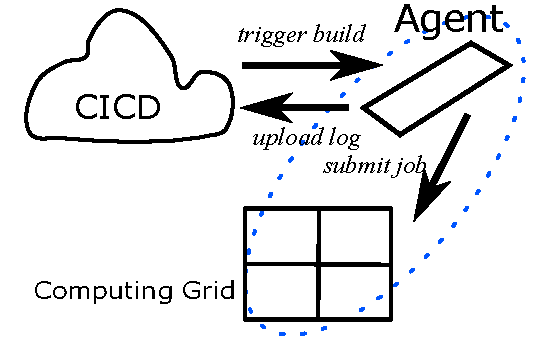
\includegraphics[width=18.5pc]{self-hosted.pdf}}
\caption{Using self-hosted HPC to connect DevOps server. The blue ellipse part is self-hosted resources.}\label{fig:selfhosted}
\end{figure}

We make a simple experiment which uses OpenMP to parallel the program. The complexity depends on the scale of input data. For two kinds of input data, the detail is shown in {\bf Table} \ref{tab:time}.
\begin{table}
\centering
\begin{tabular}{|c|p{1.5cm}|p{1.5cm}|}
\hline
Data Size & 527 MB & 2.0 GB\\
\hline
Data Source & Git LFS & HPC Storage Node \\
\hline
Platform & Travis Public Agent & HPC Computing Node  \\
\hline
CPU Core & 2 & 32  \\ 
\hline
Peak Memory  & 3.1 GB  & 17.9 GB\\ 
\hline
Time & 4.3 Minutes & 10.5 Hours \\
\hline
\end{tabular}
\caption{Running requirement of a sample OpenMP program for different size of data}\label{tab:time}
\end{table}

The program is compiled from the same source code. We run a medium-sized experiment on the freely-available cloud server and the full experiment is run on self-hosted agent. For public available Cloud DevOps server, we download the data from git large file storage server and for lab HPC server, we save the data on local storage node. The latter experiment cannot be run on Cloud DevOps server since their virtual machine is not equipped with enough resources. But we connect the HPC head node (DevOps agent) with GitLab and the experiment is triggered by updating source code to GitLab.
These combination increases the reproducibility of the project.

For self-hosted case, storing data is much more obvious but using the absolute path may let the experiment hard to reproduce by others. Also, it is not transparent if loading data directly from self-hosted disk because others do not know whether it is original data or not. Checksum is a good way to guarantee this. We recommend researchers to verify the checksums of the data to the precomputed ground truth whether the data is downloaded freshly or loaded from cache. By guaranteeing the data integrity can the experiment be more rigorous and convincing.

% introduce run the time complexity experiment on the self-hosted server

% graph computation experiment, focues on parallel power and HPC cluster usage

\section{CONCLUSION}
DevOps infrastructure is actively maintained by software engineering community and evolves towards better usability. It will be beneficial for scientists if they could incorporate DevOps into their daily research. Researchers can run their medium-sized or partial version of experiments directly on public DevOps service and complete their full experiment using self-hosted agent. Currently, it is unknown the accessibility of DevOps by scientific community beyond scientific software development. Since DevOps is easily configurable and compatible with existing tools, we believe it will sweep more disciplines in the future.

\section{ACKNOWLEDGMENT}

This work is supported by the Natural Science Foundation of China 61807021, Shenzhen Science and Technology Research and Development Funds (JCYJ20170818094022586), and Innovation and entrepreneurship project for overseas high-level talents of Shenzhen (KQJSCX20180327144037831).


\bibliographystyle{IEEEtran}
\bibliography{exportlist}



\begin{IEEEbiography}{Feng Zhao}{\,} is
currently with Tsinghua University, PR. China. He received the B.S. degree and is pursing Ph.D degree at Department of Electronic Engineering. His research interest focus on machine learning, graph computing and scientific computing. Contact him at zhaof17@mails.tsinghua.edu.cn.
\end{IEEEbiography}

\begin{IEEEbiography}{Shaolun Huang,}{\,}is a Professor with Tsinghua-Berkley Shenzhen Institute. Contact him at shaolun.huang@sz.tsinghua.edu.cn.
\end{IEEEbiography}

\begin{IEEEbiography}{Lin Zhang,}{\,}is a Professor with Tsinghua Shenzhen International Graduate School. Contact him at linzhang@tsinghua.edu.cn.
\end{IEEEbiography}

\end{document}

